\documentclass[a4paper,12pt]{article}
\usepackage[ukrainian,english]{babel}
\usepackage{ucs}
\usepackage[utf8]{inputenc}
\usepackage[T2A]{fontenc}
\usepackage{graphicx}
\usepackage{wrapfig}
\begin{document}
\title{Моделі сучасної фізики}
\maketitle
\date{ }
<математичні моделі взаємодії матеріальних об'єктів і будови матерії>

\newpage
\tableofcontents
\newpage
\section{Лекція 1 (Вступ)}
\textbf{В.1. Сучасна модель будови Всесвіту}

\textbf{макросвіт}(елементарні частки, ядра, атоми)$\rightarrow$\textbf{мікросвіт}(окремі зікрки і системи планет)$\rightarrow$\textbf{мегасвіт}(скупчення зірок, галактики, скупчення галактик, Всесвіт в цілому)

Наука, що вивчає походження і будову Всесвіту має назву "Космологія".
Наша галактика: Галактика, або "Чумацький шлях".
\\"the Big Bang" - великий "вибух": $\Delta t\approx 13\cdot 10^9 \textrm{ років}, \approx 10^{26}\textrm{ м}.$
\\Розширення Всесвіту, з. Хаббла: $V=Hr$; галактики - свого роду "атоми" Всесвіту, розбігання галактик.
Будь-яка галактіка - гравітаційно зв'язана система зірок, занурених у газі "темну матерію", природа якої, поки що, невідома. Форми галактик: неправильні, сферичні, елісоїдні, спіральні, кульові.\\
Наша галактика:

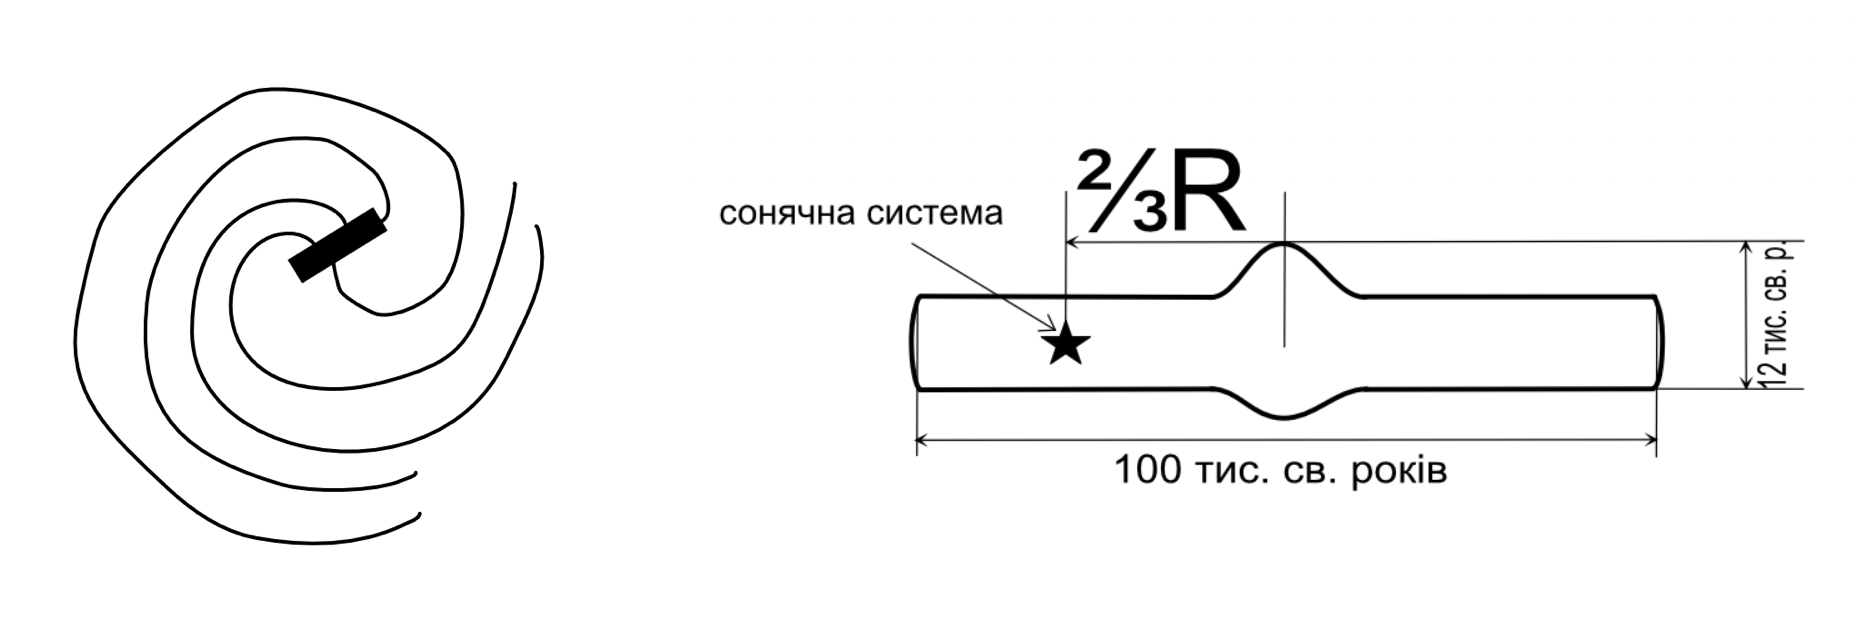
\includegraphics[width=0.7\textwidth]{galaxy0}

$\approx  10^{11}$ зірок, у Всесвіті $\sim 10^{10}$. 1 св. рік $\approx 10^{16}$м. св. рік $3,11\cdot10^7$ c; "с" $= 3\cdot10^8$. Галактики обретаются. Типовий розмір $\sim 10^{20}$ м.
\\
п'ять рукавів:
Лебедя, Оріона, Персея, Стрільця, Центаври.


Мегамиром "править" гравітаційна сила та "темна енергія". Гравітація - властивість 4-вимірного простору\\(Ейнштейн)($F=-G\frac{m_1m_2}{r^2}$ у механіці Ньютона). Сонце обертается навколо галактики: $v\approx 250$ км/с, $M_0=2\cdot10^{30}$ кг, $R_0=700$ тис. км., розмір сонячной системи $\approx 10^{13}$ м. Нейтронні зірки(як правило - пульсари), чорні діри $R=\frac{2GM}{c^2}$ - грав. радіус., $M=1,5M_0$, $R\aprrox10$ км, яблуко $\sim 20$ млн.г.

Існує 4 типи взаємодії: сильна - 1, слабка - $10^{-14}$, електромагнітна - $10^{-2}$, гравітаційна $10^{-39}$; слабка + електромагнітна - електрослабка $\approx$ 3 типи взаємодії + невідома "темна енергія"(нне плутати  темною матерією)
\end{document}
